\documentclass[conference]{IEEEtran}
\IEEEoverridecommandlockouts
% The preceding line is only needed to identify funding in the first footnote. If that is unneeded, please comment it out.
\usepackage{cite}
\usepackage{amsmath,amssymb,amsfonts}
\usepackage{algorithmic}
\usepackage{graphicx}
\usepackage{textcomp}
\usepackage{xcolor}
\usepackage{tikz}
\usepackage{hyperref}

\def\BibTeX{{\rm B\kern-.05em{\sc i\kern-.025em b}\kern-.08em
    T\kern-.1667em\lower.7ex\hbox{E}\kern-.125emX}}
\begin{document}

\title{TensorStencil Report}

\author{\IEEEauthorblockN{Robert Buxton}
\IEEEauthorblockA{rb419@ic.ac.uk}

}

\maketitle

\begin{abstract}
Todo
\end{abstract}

\begin{IEEEkeywords}
Todo
\end{IEEEkeywords}


\section{Introduction}
Todo (Make better use of tensor cores/gpu matrix multipliers for stencil computation)
\section{Method}
I propose an alternative to the classical iterative loop method for stencil computation. 
Using the emergent properties of the transformation matrices use to represent stencil time step update we can calculate the state of input data after an arbitrary number of time steps. 

SOURCE THE PAPER BEFORE THE DIAGRAM \\

\newcommand{\gridCellWidth}{0.3}
\newcommand{\gridSize}{7}
\newcommand{\gridSpacing}{0.9}
\newcommand{\gridWidth}{\gridSize*\gridCellWidth}
\definecolor{myGreen}{RGB}{95,173,86}
\definecolor{myYellow}{RGB}{242,193,78}
\definecolor{myOrange}{RGB}{247,129,84}
\newcommand{\gridAxisHorizontalCellColour}{myGreen}
\newcommand{\gridAxisVerticalCellColour}{myOrange}
\newcommand{\gridAxisMiddleColour}{myYellow}
\newcommand{\gridTwoStart}{\gridWidth + \gridSpacing}
\newcommand{\gridThreeStart}{2*\gridWidth + 2*\gridSpacing}

\begin{tikzpicture}[every node/.style={minimum size=\gridCellWidth cm-\pgflinewidth, outer sep=0pt}]

%Grid 1

\draw[step=\gridCellWidth cm,color=black] (0,0) grid (\gridWidth,\gridWidth);

\node[fill={\gridAxisHorizontalCellColour}] at (1.5*\gridCellWidth,3.5*\gridCellWidth){};
\node[fill={\gridAxisHorizontalCellColour}] at (2.5*\gridCellWidth,3.5*\gridCellWidth){};
\node[fill={\gridAxisHorizontalCellColour}] at (4.5*\gridCellWidth,3.5*\gridCellWidth){};
\node[fill={\gridAxisHorizontalCellColour}] at (5.5*\gridCellWidth,3.5*\gridCellWidth){};


\node at (1.5*\gridCellWidth,3.5*\gridCellWidth) {\footnotesize x1};
\node at (2.5*\gridCellWidth,3.5*\gridCellWidth) {\footnotesize x2};
\node at (4.5*\gridCellWidth,3.5*\gridCellWidth) {\footnotesize x3};
\node at (5.5*\gridCellWidth,3.5*\gridCellWidth) {\footnotesize x4};


\node[fill={\gridAxisVerticalCellColour}] at (3.5*\gridCellWidth,1.5*\gridCellWidth){};
\node[fill={\gridAxisVerticalCellColour}] at (3.5*\gridCellWidth,2.5*\gridCellWidth){};
\node[fill={\gridAxisVerticalCellColour}] at (3.5*\gridCellWidth,4.5*\gridCellWidth){};
\node[fill={\gridAxisVerticalCellColour}] at (3.5*\gridCellWidth,5.5*\gridCellWidth){};

\node at (3.5*\gridCellWidth,1.5*\gridCellWidth) {\footnotesize y4};
\node at (3.5*\gridCellWidth,2.5*\gridCellWidth) {\footnotesize y3};
\node at (3.5*\gridCellWidth,4.5*\gridCellWidth) {\footnotesize y2};
\node at (3.5*\gridCellWidth,5.5*\gridCellWidth) {\footnotesize y1};


\node[fill={\gridAxisMiddleColour}] at (3.5*\gridCellWidth,3.5*\gridCellWidth){};

\node at (3.5*\gridCellWidth,3.5*\gridCellWidth) {\footnotesize m};

\node[fill={\gridAxisMiddleColour}] at (\gridTwoStart + 3.5*\gridCellWidth,3.5*\gridCellWidth){};
\node at (\gridTwoStart + 3.5*\gridCellWidth,3.5*\gridCellWidth) {\tiny{$\frac{\text{m}}{2}$} };

%Grid 2

\draw[step=\gridCellWidth cm,color=black] (\gridThreeStart,0) grid (\gridWidth + \gridThreeStart,\gridWidth);

\node[fill={\gridAxisVerticalCellColour}] at (\gridTwoStart + 3.5*\gridCellWidth,2.5*\gridCellWidth){};
\node[fill={\gridAxisVerticalCellColour}] at (\gridTwoStart + 3.5*\gridCellWidth,1.5*\gridCellWidth){};
\node[fill={\gridAxisVerticalCellColour}] at (\gridTwoStart + 3.5*\gridCellWidth,4.5*\gridCellWidth){};
\node[fill={\gridAxisVerticalCellColour}] at (\gridTwoStart + 3.5*\gridCellWidth,5.5*\gridCellWidth){};

\node at (\gridTwoStart + 3.5*\gridCellWidth,1.5*\gridCellWidth) {\footnotesize y4};
\node at (\gridTwoStart + 3.5*\gridCellWidth,2.5*\gridCellWidth) {\footnotesize y3};
\node at (\gridTwoStart + 3.5*\gridCellWidth,4.5*\gridCellWidth) {\footnotesize y2};
\node at (\gridTwoStart + 3.5*\gridCellWidth,5.5*\gridCellWidth) {\footnotesize y1};

%Grid 3

\draw[step=\gridCellWidth cm,color=black] (\gridTwoStart,0) grid (\gridWidth + \gridTwoStart,\gridWidth);

\node[fill={\gridAxisHorizontalCellColour}] at (\gridThreeStart + 1.5*\gridCellWidth,3.5*\gridCellWidth){};
\node[fill={\gridAxisHorizontalCellColour}] at (\gridThreeStart + 2.5*\gridCellWidth,3.5*\gridCellWidth){};
\node[fill={\gridAxisHorizontalCellColour}] at (\gridThreeStart + 4.5*\gridCellWidth,3.5*\gridCellWidth){};
\node[fill={\gridAxisHorizontalCellColour}] at (\gridThreeStart + 5.5*\gridCellWidth,3.5*\gridCellWidth){};

\node at (\gridThreeStart + 1.5*\gridCellWidth,3.5*\gridCellWidth) {\footnotesize x1};
\node at (\gridThreeStart + 2.5*\gridCellWidth,3.5*\gridCellWidth) {\footnotesize x2};
\node at (\gridThreeStart + 4.5*\gridCellWidth,3.5*\gridCellWidth) {\footnotesize x3};
\node at (\gridThreeStart + 5.5*\gridCellWidth,3.5*\gridCellWidth) {\footnotesize x4};


\node[fill={\gridAxisMiddleColour}] at (\gridThreeStart + 3.5*\gridCellWidth,3.5*\gridCellWidth){};
\node at (\gridThreeStart + 3.5*\gridCellWidth,3.5*\gridCellWidth) {\tiny{$\frac{\text{m}}{2}$} };


\node at (\gridWidth + \gridSpacing/2 ,3.5*\gridCellWidth){\large =};
\node at (\gridThreeStart - \gridSpacing/2 ,3.5*\gridCellWidth){\large +};

\end{tikzpicture} \\
\renewcommand{\gridCellWidth}{0.3}
\renewcommand{\gridSize}{7}
\renewcommand{\gridSpacing}{0.9}
\renewcommand{\gridWidth}{\gridSize*\gridCellWidth}
\renewcommand{\gridTwoStart}{\gridWidth + \gridSpacing}

\begin{tikzpicture}[every node/.style={minimum size=\gridCellWidth cm-\pgflinewidth, outer sep=0pt}]

%Grid 1

\draw[step=\gridCellWidth cm,color=black] (0,0) grid (\gridWidth,\gridWidth);

\node[fill={\gridAxisVerticalCellColour}] at (3.5*\gridCellWidth,1.5*\gridCellWidth){};
\node[fill={\gridAxisVerticalCellColour}] at (3.5*\gridCellWidth,2.5*\gridCellWidth){};
\node[fill={\gridAxisVerticalCellColour}] at (3.5*\gridCellWidth,4.5*\gridCellWidth){};
\node[fill={\gridAxisVerticalCellColour}] at (3.5*\gridCellWidth,5.5*\gridCellWidth){};

\node at (3.5*\gridCellWidth,1.5*\gridCellWidth) {\footnotesize y4};
\node at (3.5*\gridCellWidth,2.5*\gridCellWidth) {\footnotesize y3};
\node at (3.5*\gridCellWidth,4.5*\gridCellWidth) {\footnotesize y2};
\node at (3.5*\gridCellWidth,5.5*\gridCellWidth) {\footnotesize y1};

\node[fill={\gridAxisMiddleColour}] at (3.5*\gridCellWidth,3.5*\gridCellWidth){};

\node at (3.5*\gridCellWidth,3.5*\gridCellWidth) {\tiny{$\frac{\text{m}}{2}$}};

%Grid 2

\draw[step=\gridCellWidth cm,color=black] (\gridTwoStart,0) grid (\gridWidth + \gridTwoStart,\gridWidth);

\node[fill={\gridAxisVerticalCellColour}] at (\gridTwoStart + 0.5*\gridCellWidth,4.5*\gridCellWidth) {};
\node[fill={\gridAxisVerticalCellColour}] at (\gridTwoStart + 1.5*\gridCellWidth,3.5*\gridCellWidth) {};
\node[fill={\gridAxisVerticalCellColour}] at (\gridTwoStart + 2.5*\gridCellWidth,2.5*\gridCellWidth) {};
\node[fill={\gridAxisVerticalCellColour}] at (\gridTwoStart + 3.5*\gridCellWidth,1.5*\gridCellWidth) {};
\node[fill={\gridAxisVerticalCellColour}] at (\gridTwoStart + 4.5*\gridCellWidth,0.5*\gridCellWidth) {};

\node at (\gridTwoStart + 0.5*\gridCellWidth,4.5*\gridCellWidth) {\footnotesize y1};
\node at (\gridTwoStart + 1.5*\gridCellWidth,3.5*\gridCellWidth) {\footnotesize y1};
\node at (\gridTwoStart + 2.5*\gridCellWidth,2.5*\gridCellWidth) {\footnotesize y1};
\node at (\gridTwoStart + 3.5*\gridCellWidth,1.5*\gridCellWidth) {\footnotesize y1};
\node at (\gridTwoStart + 4.5*\gridCellWidth,0.5*\gridCellWidth) {\footnotesize y1};


\node[fill={\gridAxisVerticalCellColour}] at (\gridTwoStart + 0.5*\gridCellWidth,5.5*\gridCellWidth) {};
\node[fill={\gridAxisVerticalCellColour}] at (\gridTwoStart + 1.5*\gridCellWidth,4.5*\gridCellWidth) {};
\node[fill={\gridAxisVerticalCellColour}] at (\gridTwoStart + 2.5*\gridCellWidth,3.5*\gridCellWidth) {};
\node[fill={\gridAxisVerticalCellColour}] at (\gridTwoStart + 3.5*\gridCellWidth,2.5*\gridCellWidth) {};
\node[fill={\gridAxisVerticalCellColour}] at (\gridTwoStart + 4.5*\gridCellWidth,1.5*\gridCellWidth) {};
\node[fill={\gridAxisVerticalCellColour}] at (\gridTwoStart + 5.5*\gridCellWidth,0.5*\gridCellWidth) {};

\node at (\gridTwoStart + 0.5*\gridCellWidth,5.5*\gridCellWidth) {\footnotesize y2};
\node at (\gridTwoStart + 1.5*\gridCellWidth,4.5*\gridCellWidth) {\footnotesize y2};
\node at (\gridTwoStart + 2.5*\gridCellWidth,3.5*\gridCellWidth) {\footnotesize y2};
\node at (\gridTwoStart + 3.5*\gridCellWidth,2.5*\gridCellWidth) {\footnotesize y2};
\node at (\gridTwoStart + 4.5*\gridCellWidth,1.5*\gridCellWidth) {\footnotesize y2};
\node at (\gridTwoStart + 5.5*\gridCellWidth,0.5*\gridCellWidth) {\footnotesize y2};


\node[fill={\gridAxisMiddleColour}] at (\gridTwoStart + 0.5*\gridCellWidth,6.5*\gridCellWidth){};
\node[fill={\gridAxisMiddleColour}] at (\gridTwoStart + 1.5*\gridCellWidth,5.5*\gridCellWidth){};
\node[fill={\gridAxisMiddleColour}] at (\gridTwoStart + 2.5*\gridCellWidth,4.5*\gridCellWidth){};
\node[fill={\gridAxisMiddleColour}] at (\gridTwoStart + 3.5*\gridCellWidth,3.5*\gridCellWidth){};
\node[fill={\gridAxisMiddleColour}] at (\gridTwoStart + 4.5*\gridCellWidth,2.5*\gridCellWidth){};
\node[fill={\gridAxisMiddleColour}] at (\gridTwoStart + 5.5*\gridCellWidth,1.5*\gridCellWidth){};
\node[fill={\gridAxisMiddleColour}] at (\gridTwoStart + 6.5*\gridCellWidth,0.5*\gridCellWidth){};

\node at (\gridTwoStart + 0.5*\gridCellWidth,6.5*\gridCellWidth) {\tiny{$\frac{\text{m}}{2}$} };
\node at (\gridTwoStart + 1.5*\gridCellWidth,5.5*\gridCellWidth) {\tiny{$\frac{\text{m}}{2}$} };
\node at (\gridTwoStart + 2.5*\gridCellWidth,4.5*\gridCellWidth) {\tiny{$\frac{\text{m}}{2}$} };
\node at (\gridTwoStart + 3.5*\gridCellWidth,3.5*\gridCellWidth) {\tiny{$\frac{\text{m}}{2}$} };
\node at (\gridTwoStart + 4.5*\gridCellWidth,2.5*\gridCellWidth) {\tiny{$\frac{\text{m}}{2}$} };
\node at (\gridTwoStart + 5.5*\gridCellWidth,1.5*\gridCellWidth) {\tiny{$\frac{\text{m}}{2}$} };
\node at (\gridTwoStart + 6.5*\gridCellWidth,0.5*\gridCellWidth) {\tiny{$\frac{\text{m}}{2}$} };


\node[fill={\gridAxisVerticalCellColour}] at (\gridTwoStart + 1.5*\gridCellWidth,6.5*\gridCellWidth) {};
\node[fill={\gridAxisVerticalCellColour}] at (\gridTwoStart + 2.5*\gridCellWidth,5.5*\gridCellWidth) {};
\node[fill={\gridAxisVerticalCellColour}] at (\gridTwoStart + 3.5*\gridCellWidth,4.5*\gridCellWidth) {};
\node[fill={\gridAxisVerticalCellColour}] at (\gridTwoStart + 4.5*\gridCellWidth,3.5*\gridCellWidth) {};
\node[fill={\gridAxisVerticalCellColour}] at (\gridTwoStart + 5.5*\gridCellWidth,2.5*\gridCellWidth) {};
\node[fill={\gridAxisVerticalCellColour}] at (\gridTwoStart + 6.5*\gridCellWidth,1.5*\gridCellWidth) {};

\node at (\gridTwoStart + 1.5*\gridCellWidth,6.5*\gridCellWidth) {\footnotesize y3};
\node at (\gridTwoStart + 2.5*\gridCellWidth,5.5*\gridCellWidth) {\footnotesize y3};
\node at (\gridTwoStart + 3.5*\gridCellWidth,4.5*\gridCellWidth) {\footnotesize y3};
\node at (\gridTwoStart + 4.5*\gridCellWidth,3.5*\gridCellWidth) {\footnotesize y3};
\node at (\gridTwoStart + 5.5*\gridCellWidth,2.5*\gridCellWidth) {\footnotesize y3};
\node at (\gridTwoStart + 6.5*\gridCellWidth,1.5*\gridCellWidth) {\footnotesize y3};


\node[fill={\gridAxisVerticalCellColour}] at (\gridTwoStart + 2.5*\gridCellWidth,6.5*\gridCellWidth) {};
\node[fill={\gridAxisVerticalCellColour}] at (\gridTwoStart + 3.5*\gridCellWidth,5.5*\gridCellWidth) {};
\node[fill={\gridAxisVerticalCellColour}] at (\gridTwoStart + 4.5*\gridCellWidth,4.5*\gridCellWidth) {};
\node[fill={\gridAxisVerticalCellColour}] at (\gridTwoStart + 5.5*\gridCellWidth,3.5*\gridCellWidth) {};
\node[fill={\gridAxisVerticalCellColour}] at (\gridTwoStart + 6.5*\gridCellWidth,2.5*\gridCellWidth) {};

\node at (\gridTwoStart + 2.5*\gridCellWidth,6.5*\gridCellWidth) {\footnotesize y4};
\node at (\gridTwoStart + 3.5*\gridCellWidth,5.5*\gridCellWidth) {\footnotesize y4};
\node at (\gridTwoStart + 4.5*\gridCellWidth,4.5*\gridCellWidth) {\footnotesize y4};
\node at (\gridTwoStart + 5.5*\gridCellWidth,3.5*\gridCellWidth) {\footnotesize y4};
\node at (\gridTwoStart + 6.5*\gridCellWidth,2.5*\gridCellWidth) {\footnotesize y4};


% X and ->
\node at (\gridWidth + \gridSpacing/2 ,3.5*\gridCellWidth){\large $\rightarrow$};
\node at (\gridTwoStart + \gridWidth + \gridSpacing/2 ,3.5*\gridCellWidth){\large $\quad = Y $};


\end{tikzpicture} \\
\renewcommand{\gridCellWidth}{0.3}
\renewcommand{\gridSize}{7}
\renewcommand{\gridSpacing}{0.9}
\renewcommand{\gridWidth}{\gridSize*\gridCellWidth}
\renewcommand{\gridTwoStart}{\gridWidth + \gridSpacing}

\begin{tikzpicture}[every node/.style={minimum size=\gridCellWidth cm-\pgflinewidth, outer sep=0pt}]

%Grid 1

\draw[step=\gridCellWidth cm,color=black] (0,0) grid (\gridWidth,\gridWidth);

\node[fill={\gridAxisHorizontalCellColour}] at (1.5*\gridCellWidth,3.5*\gridCellWidth){};
\node[fill={\gridAxisHorizontalCellColour}] at (2.5*\gridCellWidth,3.5*\gridCellWidth){};
\node[fill={\gridAxisHorizontalCellColour}] at (4.5*\gridCellWidth,3.5*\gridCellWidth){};
\node[fill={\gridAxisHorizontalCellColour}] at (5.5*\gridCellWidth,3.5*\gridCellWidth){};

\node at (1.5*\gridCellWidth,3.5*\gridCellWidth) {\footnotesize x1};
\node at (2.5*\gridCellWidth,3.5*\gridCellWidth) {\footnotesize x2};
\node at (4.5*\gridCellWidth,3.5*\gridCellWidth) {\footnotesize x3};
\node at (5.5*\gridCellWidth,3.5*\gridCellWidth) {\footnotesize x4};

\node[fill={\gridAxisMiddleColour}] at (3.5*\gridCellWidth,3.5*\gridCellWidth){};

\node at (3.5*\gridCellWidth,3.5*\gridCellWidth) {\tiny{$\frac{\text{m}}{2}$}};

%Grid 2

\draw[step=\gridCellWidth cm,color=black] (\gridTwoStart,0) grid (\gridWidth + \gridTwoStart,\gridWidth);

\node[fill={\gridAxisHorizontalCellColour}] at (\gridTwoStart + 0.5*\gridCellWidth,4.5*\gridCellWidth) {};
\node[fill={\gridAxisHorizontalCellColour}] at (\gridTwoStart + 1.5*\gridCellWidth,3.5*\gridCellWidth) {};
\node[fill={\gridAxisHorizontalCellColour}] at (\gridTwoStart + 2.5*\gridCellWidth,2.5*\gridCellWidth) {};
\node[fill={\gridAxisHorizontalCellColour}] at (\gridTwoStart + 3.5*\gridCellWidth,1.5*\gridCellWidth) {};
\node[fill={\gridAxisHorizontalCellColour}] at (\gridTwoStart + 4.5*\gridCellWidth,0.5*\gridCellWidth) {};

\node at (\gridTwoStart + 0.5*\gridCellWidth,4.5*\gridCellWidth) {\footnotesize x1};
\node at (\gridTwoStart + 1.5*\gridCellWidth,3.5*\gridCellWidth) {\footnotesize x1};
\node at (\gridTwoStart + 2.5*\gridCellWidth,2.5*\gridCellWidth) {\footnotesize x1};
\node at (\gridTwoStart + 3.5*\gridCellWidth,1.5*\gridCellWidth) {\footnotesize x1};
\node at (\gridTwoStart + 4.5*\gridCellWidth,0.5*\gridCellWidth) {\footnotesize x1};


\node[fill={\gridAxisHorizontalCellColour}] at (\gridTwoStart + 0.5*\gridCellWidth,5.5*\gridCellWidth) {};
\node[fill={\gridAxisHorizontalCellColour}] at (\gridTwoStart + 1.5*\gridCellWidth,4.5*\gridCellWidth) {};
\node[fill={\gridAxisHorizontalCellColour}] at (\gridTwoStart + 2.5*\gridCellWidth,3.5*\gridCellWidth) {};
\node[fill={\gridAxisHorizontalCellColour}] at (\gridTwoStart + 3.5*\gridCellWidth,2.5*\gridCellWidth) {};
\node[fill={\gridAxisHorizontalCellColour}] at (\gridTwoStart + 4.5*\gridCellWidth,1.5*\gridCellWidth) {};
\node[fill={\gridAxisHorizontalCellColour}] at (\gridTwoStart + 5.5*\gridCellWidth,0.5*\gridCellWidth) {};

\node at (\gridTwoStart + 0.5*\gridCellWidth,5.5*\gridCellWidth) {\footnotesize x2};
\node at (\gridTwoStart + 1.5*\gridCellWidth,4.5*\gridCellWidth) {\footnotesize x2};
\node at (\gridTwoStart + 2.5*\gridCellWidth,3.5*\gridCellWidth) {\footnotesize x2};
\node at (\gridTwoStart + 3.5*\gridCellWidth,2.5*\gridCellWidth) {\footnotesize x2};
\node at (\gridTwoStart + 4.5*\gridCellWidth,1.5*\gridCellWidth) {\footnotesize x2};
\node at (\gridTwoStart + 5.5*\gridCellWidth,0.5*\gridCellWidth) {\footnotesize x2};


\node[fill={\gridAxisMiddleColour}] at (\gridTwoStart + 0.5*\gridCellWidth,6.5*\gridCellWidth){};
\node[fill={\gridAxisMiddleColour}] at (\gridTwoStart + 1.5*\gridCellWidth,5.5*\gridCellWidth){};
\node[fill={\gridAxisMiddleColour}] at (\gridTwoStart + 2.5*\gridCellWidth,4.5*\gridCellWidth){};
\node[fill={\gridAxisMiddleColour}] at (\gridTwoStart + 3.5*\gridCellWidth,3.5*\gridCellWidth){};
\node[fill={\gridAxisMiddleColour}] at (\gridTwoStart + 4.5*\gridCellWidth,2.5*\gridCellWidth){};
\node[fill={\gridAxisMiddleColour}] at (\gridTwoStart + 5.5*\gridCellWidth,1.5*\gridCellWidth){};
\node[fill={\gridAxisMiddleColour}] at (\gridTwoStart + 6.5*\gridCellWidth,0.5*\gridCellWidth){};

\node at (\gridTwoStart + 0.5*\gridCellWidth,6.5*\gridCellWidth) {\tiny{$\frac{\text{m}}{2}$} };
\node at (\gridTwoStart + 1.5*\gridCellWidth,5.5*\gridCellWidth) {\tiny{$\frac{\text{m}}{2}$} };
\node at (\gridTwoStart + 2.5*\gridCellWidth,4.5*\gridCellWidth) {\tiny{$\frac{\text{m}}{2}$} };
\node at (\gridTwoStart + 3.5*\gridCellWidth,3.5*\gridCellWidth) {\tiny{$\frac{\text{m}}{2}$} };
\node at (\gridTwoStart + 4.5*\gridCellWidth,2.5*\gridCellWidth) {\tiny{$\frac{\text{m}}{2}$} };
\node at (\gridTwoStart + 5.5*\gridCellWidth,1.5*\gridCellWidth) {\tiny{$\frac{\text{m}}{2}$} };
\node at (\gridTwoStart + 6.5*\gridCellWidth,0.5*\gridCellWidth) {\tiny{$\frac{\text{m}}{2}$} };


\node[fill={\gridAxisHorizontalCellColour}] at (\gridTwoStart + 1.5*\gridCellWidth,6.5*\gridCellWidth) {};
\node[fill={\gridAxisHorizontalCellColour}] at (\gridTwoStart + 2.5*\gridCellWidth,5.5*\gridCellWidth) {};
\node[fill={\gridAxisHorizontalCellColour}] at (\gridTwoStart + 3.5*\gridCellWidth,4.5*\gridCellWidth) {};
\node[fill={\gridAxisHorizontalCellColour}] at (\gridTwoStart + 4.5*\gridCellWidth,3.5*\gridCellWidth) {};
\node[fill={\gridAxisHorizontalCellColour}] at (\gridTwoStart + 5.5*\gridCellWidth,2.5*\gridCellWidth) {};
\node[fill={\gridAxisHorizontalCellColour}] at (\gridTwoStart + 6.5*\gridCellWidth,1.5*\gridCellWidth) {};

\node at (\gridTwoStart + 1.5*\gridCellWidth,6.5*\gridCellWidth) {\footnotesize x3};
\node at (\gridTwoStart + 2.5*\gridCellWidth,5.5*\gridCellWidth) {\footnotesize x3};
\node at (\gridTwoStart + 3.5*\gridCellWidth,4.5*\gridCellWidth) {\footnotesize x3};
\node at (\gridTwoStart + 4.5*\gridCellWidth,3.5*\gridCellWidth) {\footnotesize x3};
\node at (\gridTwoStart + 5.5*\gridCellWidth,2.5*\gridCellWidth) {\footnotesize x3};
\node at (\gridTwoStart + 6.5*\gridCellWidth,1.5*\gridCellWidth) {\footnotesize x3};


\node[fill={\gridAxisHorizontalCellColour}] at (\gridTwoStart + 2.5*\gridCellWidth,6.5*\gridCellWidth) {};
\node[fill={\gridAxisHorizontalCellColour}] at (\gridTwoStart + 3.5*\gridCellWidth,5.5*\gridCellWidth) {};
\node[fill={\gridAxisHorizontalCellColour}] at (\gridTwoStart + 4.5*\gridCellWidth,4.5*\gridCellWidth) {};
\node[fill={\gridAxisHorizontalCellColour}] at (\gridTwoStart + 5.5*\gridCellWidth,3.5*\gridCellWidth) {};
\node[fill={\gridAxisHorizontalCellColour}] at (\gridTwoStart + 6.5*\gridCellWidth,2.5*\gridCellWidth) {};

\node at (\gridTwoStart + 2.5*\gridCellWidth,6.5*\gridCellWidth) {\footnotesize x4};
\node at (\gridTwoStart + 3.5*\gridCellWidth,5.5*\gridCellWidth) {\footnotesize x4};
\node at (\gridTwoStart + 4.5*\gridCellWidth,4.5*\gridCellWidth) {\footnotesize x4};
\node at (\gridTwoStart + 5.5*\gridCellWidth,3.5*\gridCellWidth) {\footnotesize x4};
\node at (\gridTwoStart + 6.5*\gridCellWidth,2.5*\gridCellWidth) {\footnotesize x4};


% Y and ->
\node at (\gridWidth + \gridSpacing/2 ,3.5*\gridCellWidth){\large $\rightarrow$};
\node at (\gridTwoStart + \gridWidth + \gridSpacing/2 ,3.5*\gridCellWidth){\large $\quad = X $};

\end{tikzpicture} \\
\renewcommand{\gridCellWidth}{0.3}
\renewcommand{\gridSize}{7}
\renewcommand{\gridSpacing}{1.5}
\renewcommand{\gridWidth}{\gridSize*\gridCellWidth}
\renewcommand{\gridAxisHorizontalCellColour}{myGreen}
\renewcommand{\gridAxisVerticalCellColour}{myOrange}
\renewcommand{\gridAxisMiddleColour}{myYellow}
\renewcommand{\gridTwoStart}{\gridSpacing}
\renewcommand{\gridThreeStart}{\gridTwoStart + \gridWidth + \gridSpacing}



\begin{tikzpicture}[every node/.style={minimum size=\gridCellWidth cm-\pgflinewidth, outer sep=0pt}]

%Grid 1

\node at (\gridSpacing/2,3.5*\gridCellWidth) {\large $A_{t+1} =$};

%Grid 2

\draw[step=\gridCellWidth cm,color=black] (\gridTwoStart,0) grid (\gridWidth + \gridTwoStart,\gridWidth);

\node[fill={\gridAxisVerticalCellColour}] at (\gridTwoStart + 0.5*\gridCellWidth,4.5*\gridCellWidth) {};
\node[fill={\gridAxisVerticalCellColour}] at (\gridTwoStart + 1.5*\gridCellWidth,3.5*\gridCellWidth) {};
\node[fill={\gridAxisVerticalCellColour}] at (\gridTwoStart + 2.5*\gridCellWidth,2.5*\gridCellWidth) {};
\node[fill={\gridAxisVerticalCellColour}] at (\gridTwoStart + 3.5*\gridCellWidth,1.5*\gridCellWidth) {};
\node[fill={\gridAxisVerticalCellColour}] at (\gridTwoStart + 4.5*\gridCellWidth,0.5*\gridCellWidth) {};

\node at (\gridTwoStart + 0.5*\gridCellWidth,4.5*\gridCellWidth) {\footnotesize y1};
\node at (\gridTwoStart + 1.5*\gridCellWidth,3.5*\gridCellWidth) {\footnotesize y1};
\node at (\gridTwoStart + 2.5*\gridCellWidth,2.5*\gridCellWidth) {\footnotesize y1};
\node at (\gridTwoStart + 3.5*\gridCellWidth,1.5*\gridCellWidth) {\footnotesize y1};
\node at (\gridTwoStart + 4.5*\gridCellWidth,0.5*\gridCellWidth) {\footnotesize y1};


\node[fill={\gridAxisVerticalCellColour}] at (\gridTwoStart + 0.5*\gridCellWidth,5.5*\gridCellWidth) {};
\node[fill={\gridAxisVerticalCellColour}] at (\gridTwoStart + 1.5*\gridCellWidth,4.5*\gridCellWidth) {};
\node[fill={\gridAxisVerticalCellColour}] at (\gridTwoStart + 2.5*\gridCellWidth,3.5*\gridCellWidth) {};
\node[fill={\gridAxisVerticalCellColour}] at (\gridTwoStart + 3.5*\gridCellWidth,2.5*\gridCellWidth) {};
\node[fill={\gridAxisVerticalCellColour}] at (\gridTwoStart + 4.5*\gridCellWidth,1.5*\gridCellWidth) {};
\node[fill={\gridAxisVerticalCellColour}] at (\gridTwoStart + 5.5*\gridCellWidth,0.5*\gridCellWidth) {};

\node at (\gridTwoStart + 0.5*\gridCellWidth,5.5*\gridCellWidth) {\footnotesize y2};
\node at (\gridTwoStart + 1.5*\gridCellWidth,4.5*\gridCellWidth) {\footnotesize y2};
\node at (\gridTwoStart + 2.5*\gridCellWidth,3.5*\gridCellWidth) {\footnotesize y2};
\node at (\gridTwoStart + 3.5*\gridCellWidth,2.5*\gridCellWidth) {\footnotesize y2};
\node at (\gridTwoStart + 4.5*\gridCellWidth,1.5*\gridCellWidth) {\footnotesize y2};
\node at (\gridTwoStart + 5.5*\gridCellWidth,0.5*\gridCellWidth) {\footnotesize y2};


\node[fill={\gridAxisMiddleColour}] at (\gridTwoStart + 0.5*\gridCellWidth,6.5*\gridCellWidth){};
\node[fill={\gridAxisMiddleColour}] at (\gridTwoStart + 1.5*\gridCellWidth,5.5*\gridCellWidth){};
\node[fill={\gridAxisMiddleColour}] at (\gridTwoStart + 2.5*\gridCellWidth,4.5*\gridCellWidth){};
\node[fill={\gridAxisMiddleColour}] at (\gridTwoStart + 3.5*\gridCellWidth,3.5*\gridCellWidth){};
\node[fill={\gridAxisMiddleColour}] at (\gridTwoStart + 4.5*\gridCellWidth,2.5*\gridCellWidth){};
\node[fill={\gridAxisMiddleColour}] at (\gridTwoStart + 5.5*\gridCellWidth,1.5*\gridCellWidth){};
\node[fill={\gridAxisMiddleColour}] at (\gridTwoStart + 6.5*\gridCellWidth,0.5*\gridCellWidth){};

\node at (\gridTwoStart + 0.5*\gridCellWidth,6.5*\gridCellWidth) {\tiny{$\frac{\text{m}}{2}$} };
\node at (\gridTwoStart + 1.5*\gridCellWidth,5.5*\gridCellWidth) {\tiny{$\frac{\text{m}}{2}$} };
\node at (\gridTwoStart + 2.5*\gridCellWidth,4.5*\gridCellWidth) {\tiny{$\frac{\text{m}}{2}$} };
\node at (\gridTwoStart + 3.5*\gridCellWidth,3.5*\gridCellWidth) {\tiny{$\frac{\text{m}}{2}$} };
\node at (\gridTwoStart + 4.5*\gridCellWidth,2.5*\gridCellWidth) {\tiny{$\frac{\text{m}}{2}$} };
\node at (\gridTwoStart + 5.5*\gridCellWidth,1.5*\gridCellWidth) {\tiny{$\frac{\text{m}}{2}$} };
\node at (\gridTwoStart + 6.5*\gridCellWidth,0.5*\gridCellWidth) {\tiny{$\frac{\text{m}}{2}$} };


\node[fill={\gridAxisVerticalCellColour}] at (\gridTwoStart + 1.5*\gridCellWidth,6.5*\gridCellWidth) {};
\node[fill={\gridAxisVerticalCellColour}] at (\gridTwoStart + 2.5*\gridCellWidth,5.5*\gridCellWidth) {};
\node[fill={\gridAxisVerticalCellColour}] at (\gridTwoStart + 3.5*\gridCellWidth,4.5*\gridCellWidth) {};
\node[fill={\gridAxisVerticalCellColour}] at (\gridTwoStart + 4.5*\gridCellWidth,3.5*\gridCellWidth) {};
\node[fill={\gridAxisVerticalCellColour}] at (\gridTwoStart + 5.5*\gridCellWidth,2.5*\gridCellWidth) {};
\node[fill={\gridAxisVerticalCellColour}] at (\gridTwoStart + 6.5*\gridCellWidth,1.5*\gridCellWidth) {};

\node at (\gridTwoStart + 1.5*\gridCellWidth,6.5*\gridCellWidth) {\footnotesize y3};
\node at (\gridTwoStart + 2.5*\gridCellWidth,5.5*\gridCellWidth) {\footnotesize y3};
\node at (\gridTwoStart + 3.5*\gridCellWidth,4.5*\gridCellWidth) {\footnotesize y3};
\node at (\gridTwoStart + 4.5*\gridCellWidth,3.5*\gridCellWidth) {\footnotesize y3};
\node at (\gridTwoStart + 5.5*\gridCellWidth,2.5*\gridCellWidth) {\footnotesize y3};
\node at (\gridTwoStart + 6.5*\gridCellWidth,1.5*\gridCellWidth) {\footnotesize y3};


\node[fill={\gridAxisVerticalCellColour}] at (\gridTwoStart + 2.5*\gridCellWidth,6.5*\gridCellWidth) {};
\node[fill={\gridAxisVerticalCellColour}] at (\gridTwoStart + 3.5*\gridCellWidth,5.5*\gridCellWidth) {};
\node[fill={\gridAxisVerticalCellColour}] at (\gridTwoStart + 4.5*\gridCellWidth,4.5*\gridCellWidth) {};
\node[fill={\gridAxisVerticalCellColour}] at (\gridTwoStart + 5.5*\gridCellWidth,3.5*\gridCellWidth) {};
\node[fill={\gridAxisVerticalCellColour}] at (\gridTwoStart + 6.5*\gridCellWidth,2.5*\gridCellWidth) {};

\node at (\gridTwoStart + 2.5*\gridCellWidth,6.5*\gridCellWidth) {\footnotesize y4};
\node at (\gridTwoStart + 3.5*\gridCellWidth,5.5*\gridCellWidth) {\footnotesize y4};
\node at (\gridTwoStart + 4.5*\gridCellWidth,4.5*\gridCellWidth) {\footnotesize y4};
\node at (\gridTwoStart + 5.5*\gridCellWidth,3.5*\gridCellWidth) {\footnotesize y4};
\node at (\gridTwoStart + 6.5*\gridCellWidth,2.5*\gridCellWidth) {\footnotesize y4};

%Grid 3

\draw[step=\gridCellWidth cm,color=black] (\gridThreeStart,0) grid (\gridWidth + \gridThreeStart,\gridWidth);

\node[fill={\gridAxisHorizontalCellColour}] at (\gridThreeStart + 0.5*\gridCellWidth,4.5*\gridCellWidth) {};
\node[fill={\gridAxisHorizontalCellColour}] at (\gridThreeStart + 1.5*\gridCellWidth,3.5*\gridCellWidth) {};
\node[fill={\gridAxisHorizontalCellColour}] at (\gridThreeStart + 2.5*\gridCellWidth,2.5*\gridCellWidth) {};
\node[fill={\gridAxisHorizontalCellColour}] at (\gridThreeStart + 3.5*\gridCellWidth,1.5*\gridCellWidth) {};
\node[fill={\gridAxisHorizontalCellColour}] at (\gridThreeStart + 4.5*\gridCellWidth,0.5*\gridCellWidth) {};

\node at (\gridThreeStart + 0.5*\gridCellWidth,4.5*\gridCellWidth) {\footnotesize x1};
\node at (\gridThreeStart + 1.5*\gridCellWidth,3.5*\gridCellWidth) {\footnotesize x1};
\node at (\gridThreeStart + 2.5*\gridCellWidth,2.5*\gridCellWidth) {\footnotesize x1};
\node at (\gridThreeStart + 3.5*\gridCellWidth,1.5*\gridCellWidth) {\footnotesize x1};
\node at (\gridThreeStart + 4.5*\gridCellWidth,0.5*\gridCellWidth) {\footnotesize x1};

\node[fill={\gridAxisHorizontalCellColour}] at (\gridThreeStart + 0.5*\gridCellWidth,5.5*\gridCellWidth) {};
\node[fill={\gridAxisHorizontalCellColour}] at (\gridThreeStart + 1.5*\gridCellWidth,4.5*\gridCellWidth) {};
\node[fill={\gridAxisHorizontalCellColour}] at (\gridThreeStart + 2.5*\gridCellWidth,3.5*\gridCellWidth) {};
\node[fill={\gridAxisHorizontalCellColour}] at (\gridThreeStart + 3.5*\gridCellWidth,2.5*\gridCellWidth) {};
\node[fill={\gridAxisHorizontalCellColour}] at (\gridThreeStart + 4.5*\gridCellWidth,1.5*\gridCellWidth) {};
\node[fill={\gridAxisHorizontalCellColour}] at (\gridThreeStart + 5.5*\gridCellWidth,0.5*\gridCellWidth) {};

\node at (\gridThreeStart + 0.5*\gridCellWidth,5.5*\gridCellWidth) {\footnotesize x2};
\node at (\gridThreeStart + 1.5*\gridCellWidth,4.5*\gridCellWidth) {\footnotesize x2};
\node at (\gridThreeStart + 2.5*\gridCellWidth,3.5*\gridCellWidth) {\footnotesize x2};
\node at (\gridThreeStart + 3.5*\gridCellWidth,2.5*\gridCellWidth) {\footnotesize x2};
\node at (\gridThreeStart + 4.5*\gridCellWidth,1.5*\gridCellWidth) {\footnotesize x2};
\node at (\gridThreeStart + 5.5*\gridCellWidth,0.5*\gridCellWidth) {\footnotesize x2};


\node[fill={\gridAxisMiddleColour}] at (\gridThreeStart + 0.5*\gridCellWidth,6.5*\gridCellWidth){};
\node[fill={\gridAxisMiddleColour}] at (\gridThreeStart + 1.5*\gridCellWidth,5.5*\gridCellWidth){};
\node[fill={\gridAxisMiddleColour}] at (\gridThreeStart + 2.5*\gridCellWidth,4.5*\gridCellWidth){};
\node[fill={\gridAxisMiddleColour}] at (\gridThreeStart + 3.5*\gridCellWidth,3.5*\gridCellWidth){};
\node[fill={\gridAxisMiddleColour}] at (\gridThreeStart + 4.5*\gridCellWidth,2.5*\gridCellWidth){};
\node[fill={\gridAxisMiddleColour}] at (\gridThreeStart + 5.5*\gridCellWidth,1.5*\gridCellWidth){};
\node[fill={\gridAxisMiddleColour}] at (\gridThreeStart + 6.5*\gridCellWidth,0.5*\gridCellWidth){};

\node at (\gridThreeStart + 0.5*\gridCellWidth,6.5*\gridCellWidth) {\tiny{$\frac{\text{m}}{2}$} };
\node at (\gridThreeStart + 1.5*\gridCellWidth,5.5*\gridCellWidth) {\tiny{$\frac{\text{m}}{2}$} };
\node at (\gridThreeStart + 2.5*\gridCellWidth,4.5*\gridCellWidth) {\tiny{$\frac{\text{m}}{2}$} };
\node at (\gridThreeStart + 3.5*\gridCellWidth,3.5*\gridCellWidth) {\tiny{$\frac{\text{m}}{2}$} };
\node at (\gridThreeStart + 4.5*\gridCellWidth,2.5*\gridCellWidth) {\tiny{$\frac{\text{m}}{2}$} };
\node at (\gridThreeStart + 5.5*\gridCellWidth,1.5*\gridCellWidth) {\tiny{$\frac{\text{m}}{2}$} };
\node at (\gridThreeStart + 6.5*\gridCellWidth,0.5*\gridCellWidth) {\tiny{$\frac{\text{m}}{2}$} };


\node[fill={\gridAxisHorizontalCellColour}] at (\gridThreeStart + 1.5*\gridCellWidth,6.5*\gridCellWidth) {};
\node[fill={\gridAxisHorizontalCellColour}] at (\gridThreeStart + 2.5*\gridCellWidth,5.5*\gridCellWidth) {};
\node[fill={\gridAxisHorizontalCellColour}] at (\gridThreeStart + 3.5*\gridCellWidth,4.5*\gridCellWidth) {};
\node[fill={\gridAxisHorizontalCellColour}] at (\gridThreeStart + 4.5*\gridCellWidth,3.5*\gridCellWidth) {};
\node[fill={\gridAxisHorizontalCellColour}] at (\gridThreeStart + 5.5*\gridCellWidth,2.5*\gridCellWidth) {};
\node[fill={\gridAxisHorizontalCellColour}] at (\gridThreeStart + 6.5*\gridCellWidth,1.5*\gridCellWidth) {};

\node at (\gridThreeStart + 1.5*\gridCellWidth,6.5*\gridCellWidth) {\footnotesize x3};
\node at (\gridThreeStart + 2.5*\gridCellWidth,5.5*\gridCellWidth) {\footnotesize x3};
\node at (\gridThreeStart + 3.5*\gridCellWidth,4.5*\gridCellWidth) {\footnotesize x3};
\node at (\gridThreeStart + 4.5*\gridCellWidth,3.5*\gridCellWidth) {\footnotesize x3};
\node at (\gridThreeStart + 5.5*\gridCellWidth,2.5*\gridCellWidth) {\footnotesize x3};
\node at (\gridThreeStart + 6.5*\gridCellWidth,1.5*\gridCellWidth) {\footnotesize x3};


\node[fill={\gridAxisHorizontalCellColour}] at (\gridThreeStart + 2.5*\gridCellWidth,6.5*\gridCellWidth) {};
\node[fill={\gridAxisHorizontalCellColour}] at (\gridThreeStart + 3.5*\gridCellWidth,5.5*\gridCellWidth) {};
\node[fill={\gridAxisHorizontalCellColour}] at (\gridThreeStart + 4.5*\gridCellWidth,4.5*\gridCellWidth) {};
\node[fill={\gridAxisHorizontalCellColour}] at (\gridThreeStart + 5.5*\gridCellWidth,3.5*\gridCellWidth) {};
\node[fill={\gridAxisHorizontalCellColour}] at (\gridThreeStart + 6.5*\gridCellWidth,2.5*\gridCellWidth) {};

\node at (\gridThreeStart + 2.5*\gridCellWidth,6.5*\gridCellWidth) {\footnotesize x4};
\node at (\gridThreeStart + 3.5*\gridCellWidth,5.5*\gridCellWidth) {\footnotesize x4};
\node at (\gridThreeStart + 4.5*\gridCellWidth,4.5*\gridCellWidth) {\footnotesize x4};
\node at (\gridThreeStart + 5.5*\gridCellWidth,3.5*\gridCellWidth) {\footnotesize x4};
\node at (\gridThreeStart + 6.5*\gridCellWidth,2.5*\gridCellWidth) {\footnotesize x4};

%in between
\node at (\gridTwoStart + \gridWidth + \gridSpacing/2 ,3.5*\gridCellWidth){$\cdot A_t + A_t \cdot$};

% transpose
\node at (\gridThreeStart + \gridWidth + 0.2,\gridWidth){$T$};
\end{tikzpicture} \\

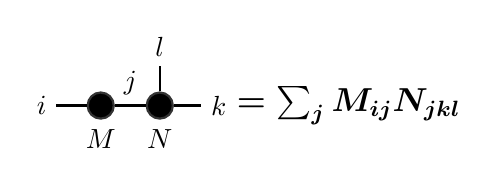
\begin{tikzpicture}
	\node[circle,draw=black!80,thick,fill=black,label=below:$M$] (M) at (0.75,0) {};
	\node[circle,draw=black!80,thick,fill=black,label=below:$N$] (N) at (1.5,0) {};
	\node (i) at (0,0) {$i$};
	\node (l) at (1.5,0.75) {$l$};
	\node (k) at (2.25,0) {$k$};
	\draw[thick, draw=black,label=above:] (M) -- node [above] {$j$} (N) {};
	\draw[thick, draw=black] (i) -- (M) {};
	\draw[thick, draw=black] (N) -- (k) {};
	\draw[thick, draw=black] (N) -- (l) {};
	\node at (3.9,0) {\large {\boldmath$= \sum_j M_{ij}N_{jkl}$}};
\end{tikzpicture}
 \\
\begin{tikzpicture}
	\node[circle,draw=black!80,thick,fill=black,label=left:$A_{t+1}$] (ATT) at (0,0) {};
	\node[circle,draw=black!80,thick,fill=black,label=left:$A_{t}$] (AT) at (2,0) {};
	\node[circle,draw=black!80,thick,fill=myGreen,label=above right:$X$] (X) at (2.5,0.5) {};
	\node[circle,draw=black!80,thick,fill=black,label=left:$A_{t}$] (A) at (4,0) {};
	\node[circle,draw=black!80,thick,fill=myOrange,label=above right:$Y$] (Y) at (4.5,-0.5) {};
	\node at (1,0) {\large $=$};
	\node at (3,0) {\large $+$};
	\draw[thick, draw=black] (ATT) -- (0,0.5) -- (0.5,0.5) {};
	\draw[thick, draw=black] (ATT) -- (0,-0.5) -- (0.5,-0.5) {};

	\draw[thick, draw=black] (AT) -- (2,0.5) -- (X) -- (3,0.5) {};
	\draw[thick, draw=black] (AT) -- (2,-0.5) -- (2.5, -0.5) {};

	\draw[thick, draw=black] (A) -- (4,0.5) -- (4.5,0.5) {};
	\draw[thick, draw=black] (A) -- (4,-0.5) -- (Y) -- (5,-0.5) {};
\end{tikzpicture}
\section{Proof}

Todo
\section{Complexity}
Todo
\section{Results}
Todo

\end{document}